\documentclass[tikz, border=10pt]{standalone}
\usepackage{pgfplots}
\pgfplotsset{compat=1.18}

% Partei-Farbcodes (RGB)
\definecolor{AfD}{RGB}{0, 158, 224}
\definecolor{CDU}{RGB}{21, 21, 24}
\definecolor{Linke}{RGB}{190, 48, 117}
\definecolor{SPD}{RGB}{227, 0, 15}
\definecolor{Gruene}{RGB}{100, 161, 45}
\definecolor{Sonstige}{RGB}{160, 160, 160}

\begin{document}
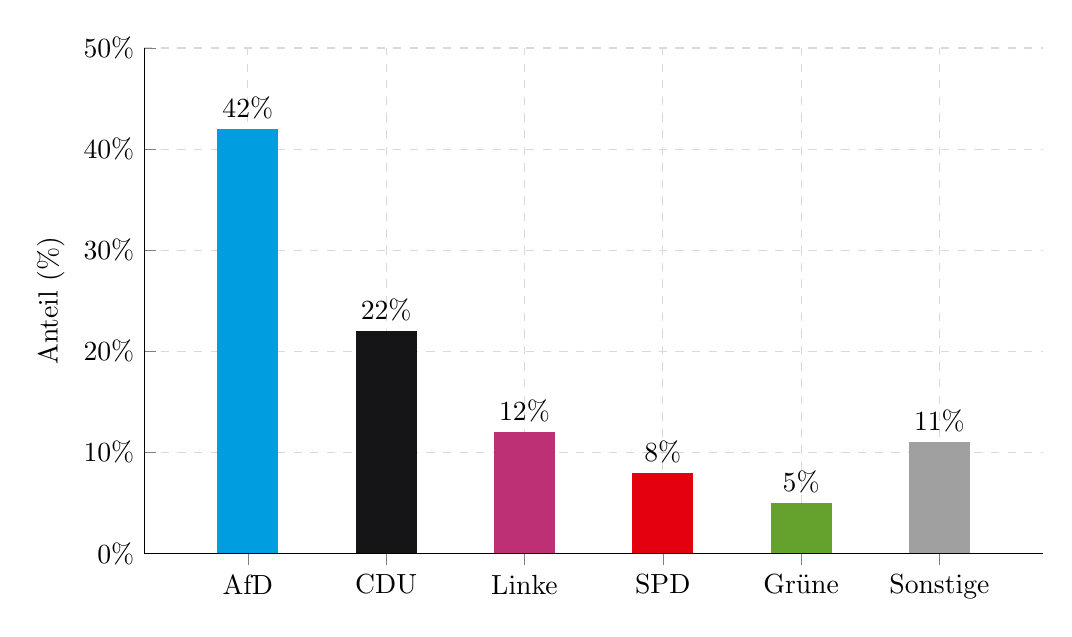
\begin{tikzpicture}
\begin{axis}[
    ybar,
    symbolic x coords={AfD, CDU, Linke, SPD, Grüne, Sonstige},
    xtick={AfD, CDU, Linke, SPD, Grüne, Sonstige},
    nodes near coords={\pgfmathprintnumber\pgfplotspointmeta\%},
    nodes near coords align={vertical},
    ymin=0, ymax=50,
    ylabel={Anteil (\%)},
    enlarge x limits=0.15,
    bar width=22pt,
    width=13cm,
    height=8cm,
    grid=major,
    grid style={dashed, gray!30},
    axis lines*=left,
    yticklabel={\pgfmathprintnumber\tick\%},
    bar shift=0pt
]

\addplot[fill=AfD, draw=none] coordinates {(AfD, 42)};
\addplot[fill=CDU, draw=none] coordinates {(CDU, 22)};
\addplot[fill=Linke, draw=none] coordinates {(Linke, 12)};
\addplot[fill=SPD, draw=none] coordinates {(SPD, 8)};
\addplot[fill=Gruene, draw=none] coordinates {(Grüne, 5)};
\addplot[fill=Sonstige, draw=none] coordinates {(Sonstige, 11)};

\end{axis}
\end{tikzpicture}
\end{document}